blah \cite{Chaiyasucheeva2012}
\section{Contributions to Knowledge}
Due to the interdisciplinary nature of my dissertation, contributions can be split into two areas: the contributions to the medical domain and the contributions to the engineering domain. The medical domain can benefit by using the WHIPPED system to test the hypothesis that engaging patients in their own self-care can lead to a better quality of life and reduce hospitalization. During the exploratory study, tests will be performed based on patients who use the traditional care method (the control), patients using only the psychosocial instruments, and patients who have the sensors and psychosocial instruments. We can also access if patients will effectively use the system to facilitate their self-care.
For the engineering domain, we will develop new and novel techniques for data fusion and knowledge acquisition supporting numerous future applications (e.g. future soldier systems, athlete training). We will design implement and validate an end-to-end system that integrates synthetic sensors, wireless communication, and the calculation of a wellness measure, using an EHR and BKE into an all-inclusive system. We will provide a medical solution to engage patients in their own self-care cheaply with little impact on the user. Our solution can reduce healthcare costs and increase quality of life. 

\begin{figure}
	\begin{center}
		\label{fig:20second}
		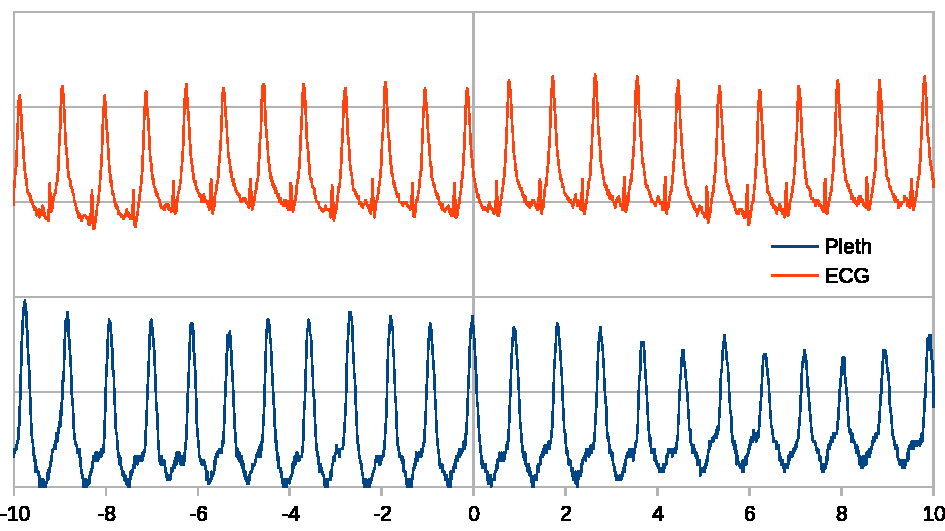
\includegraphics[scale=1,width=0.8\textwidth]{Images/20second.pdf} 
		\caption[20 second capture]{Twenty Second Captured Trace of WHIPPED Version2 ECG and SpO2 waveforms}
	\end{center}
	
\end{figure}

\begin{figure}
	\begin{center}
		\label{fig:hemoglobin}
		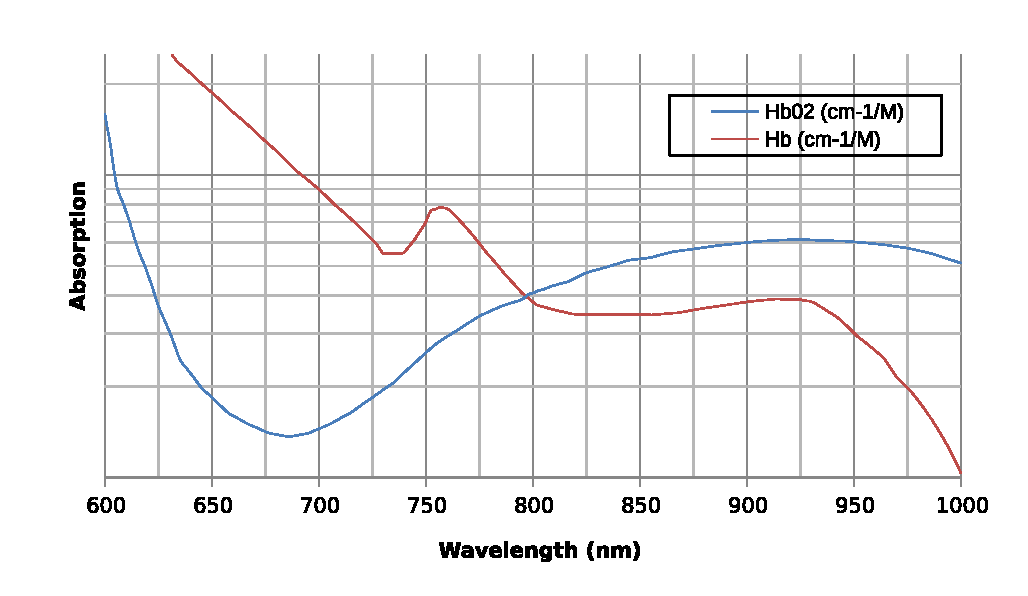
\includegraphics[scale=1,width=0.8\textwidth]{Images/hemoglobin.pdf} 
		\caption{Absorption Spectra of HbO2 (Blue) vs. Hb (Red)}
	\end{center}

\end{figure}

\begin{figure}
	\begin{center}
		\label{fig:HR69}
		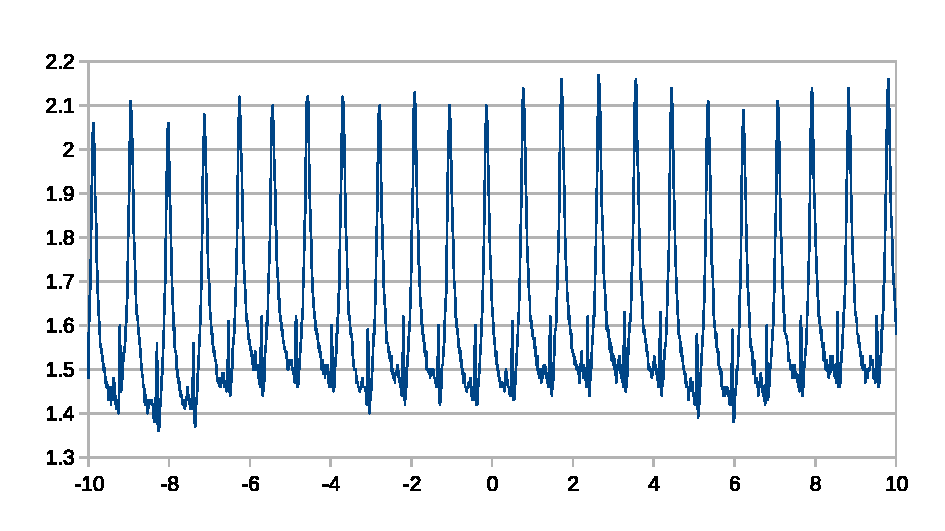
\includegraphics[scale=1,width=0.8\textwidth]{Images/HR69.pdf} 
		\caption{Sample Trace of ECG waveform with Heart Rate = 69}
	\end{center}
\end{figure}


\begin{figure}
	\begin{center}
		\label{fig:SyntheticSensor}
		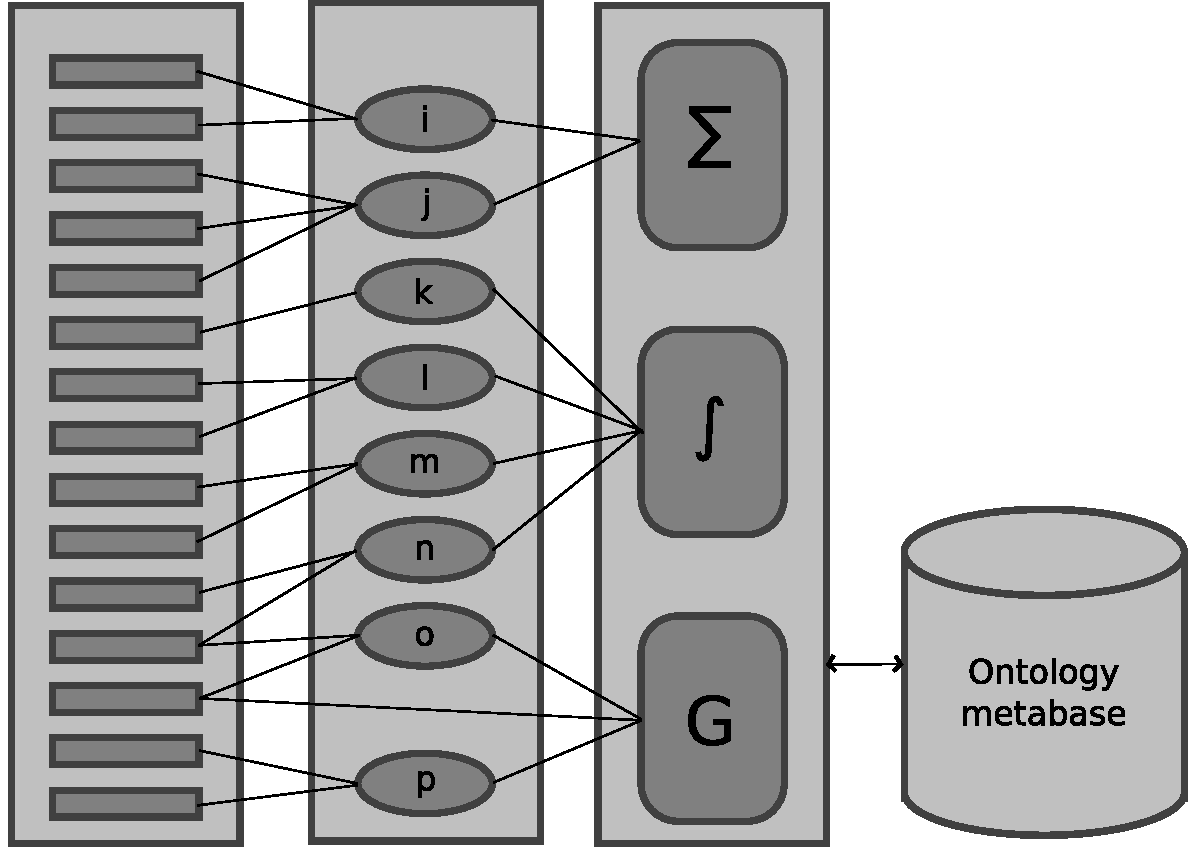
\includegraphics[scale=1,width=0.8\textwidth]{Images/syntheticSensor.pdf} 
		\caption{Synthetic Sensor Concepts for the Medical Domain}
	\end{center}
\end{figure}

\begin{figure}
	\begin{center}
		\label{fig:BasicPulse}
		%%\begin{equation}
			$\frac{23 \text{ R waves}}{20 \text{ seconds}} * \frac{60 \text{ seconds}}{1 \text{ minute}} = 69 \frac{\text{beats}}{\text{minute}}$
		%%\end{equation}
		
		\caption{Equation 1: Basic pulse rate calculation}
	\end{center}
\end{figure}


\begin{figure}
	\begin{center}
		\label{fig:42minecg}
		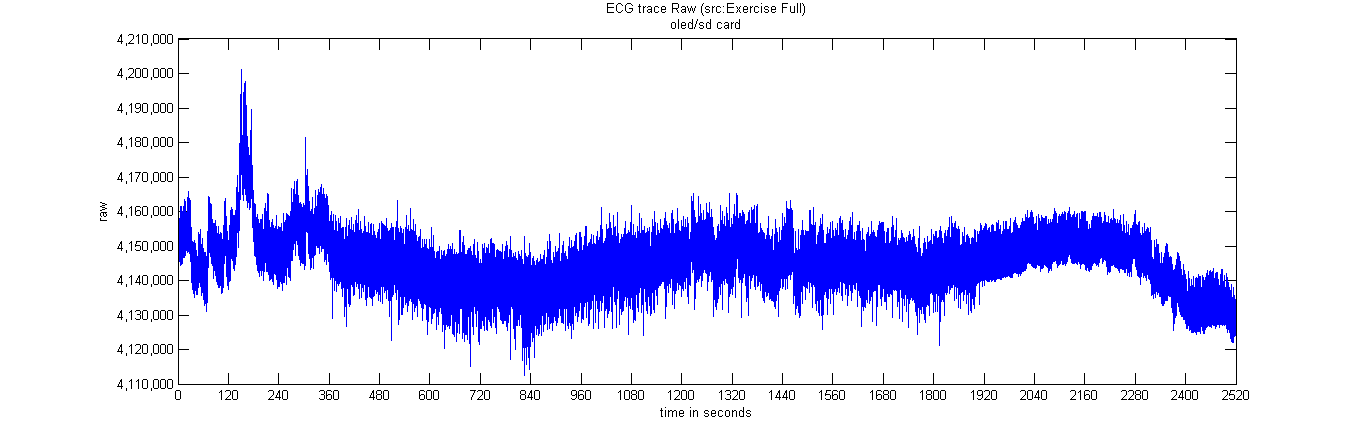
\includegraphics[scale=1,width=0.8\textwidth]{Images/42MinECGTrace.png} 
		\caption{Forty-two minute ECG trace of a twenty eight year old runner on a treadmill, with cool-down.}
	\end{center}
\end{figure}


\begin{figure}
	\begin{center}
		\label{fig:10SecRunningQRS}
		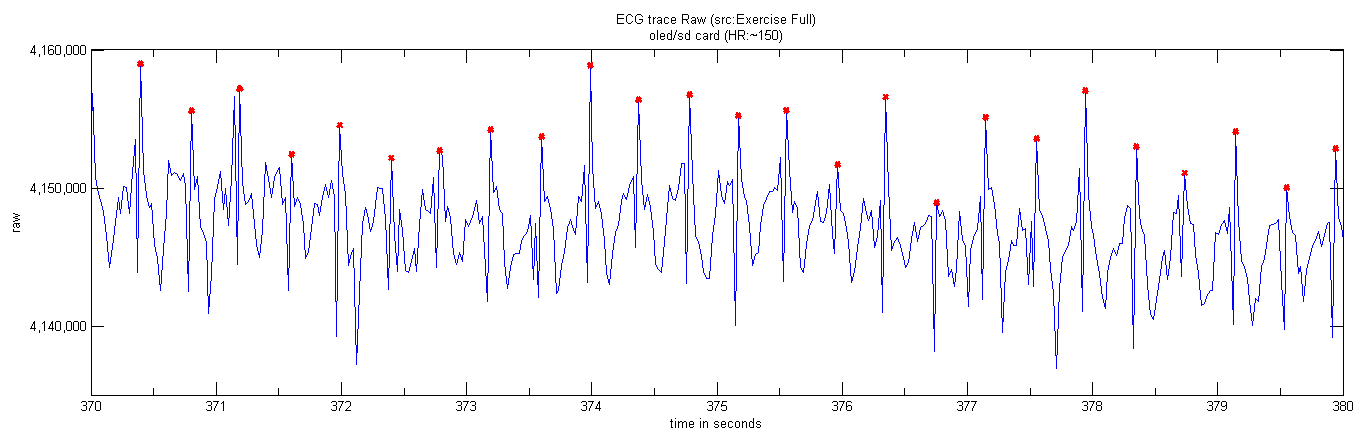
\includegraphics[scale=1,width=0.8\textwidth]{Images/10SecRunning_withQRS.png}
		\caption{Ten Second ECG trace with QRS complexes marked.}
	\end{center}
\end{figure}


\begin{figure}
	\begin{center}
		\label{fig:ecgJitter}
		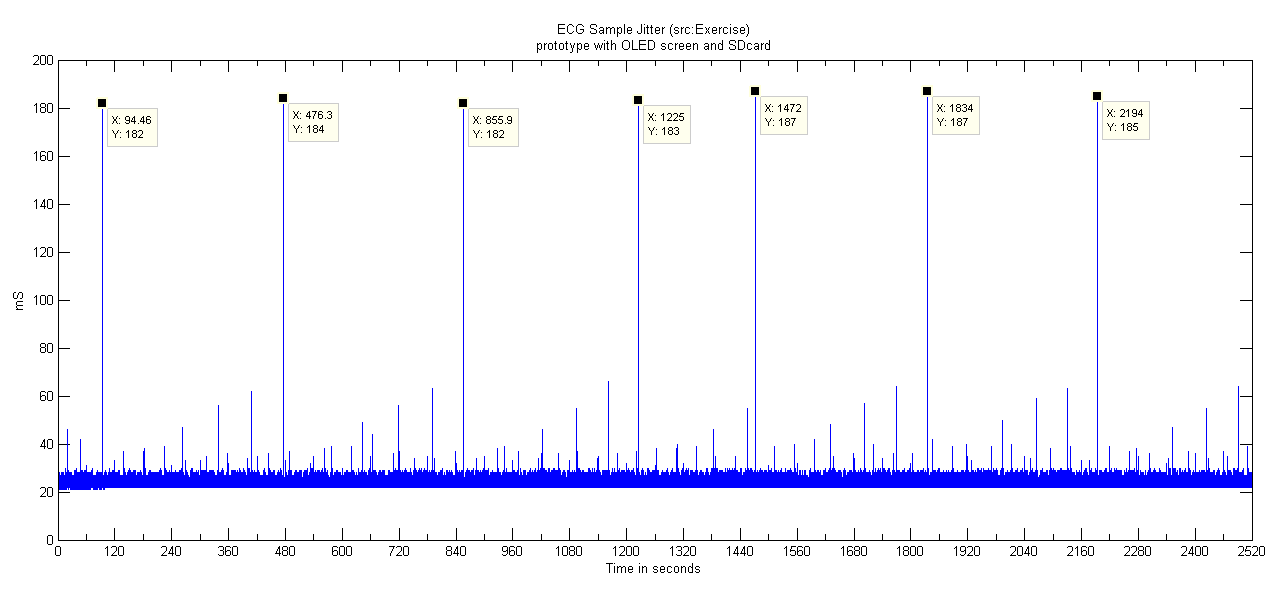
\includegraphics[scale=1,width=0.8\textwidth]{Images/ecgSampleJitter.png}
		\caption{Jitter of samples in milliseconds over time.}
	\end{center}
\end{figure}

\begin{figure}
	\begin{center}
		\label{fig:ecgJitterZoom}
		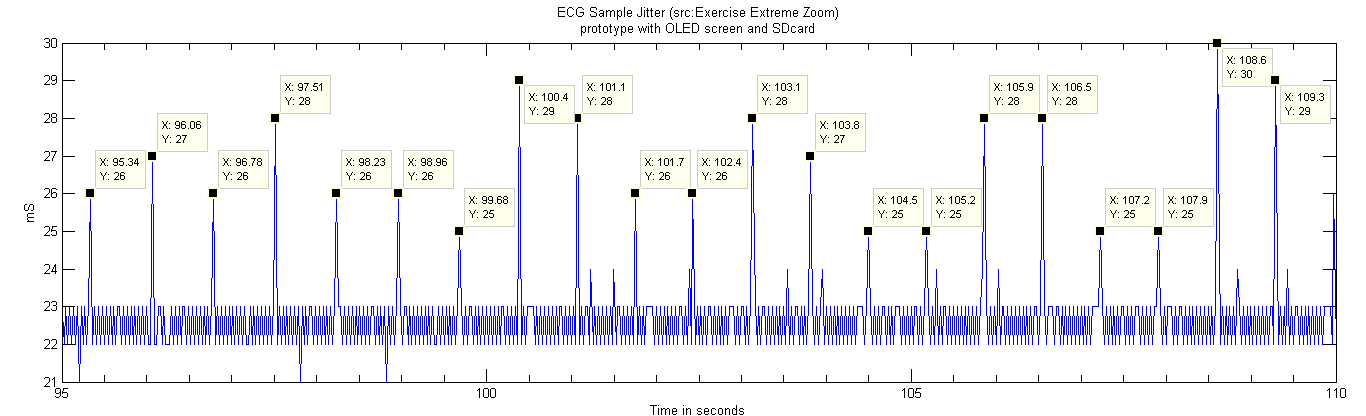
\includegraphics[scale=1,width=0.8\textwidth]{Images/ecgJitterZoom.png}
		\caption{Fifteen Second Zoom of figure 1, with abnormal jitter times marked.}
	\end{center}
\end{figure}

\begin{figure}
	\begin{center}
		\label{fig:ecgJitterZoom}
		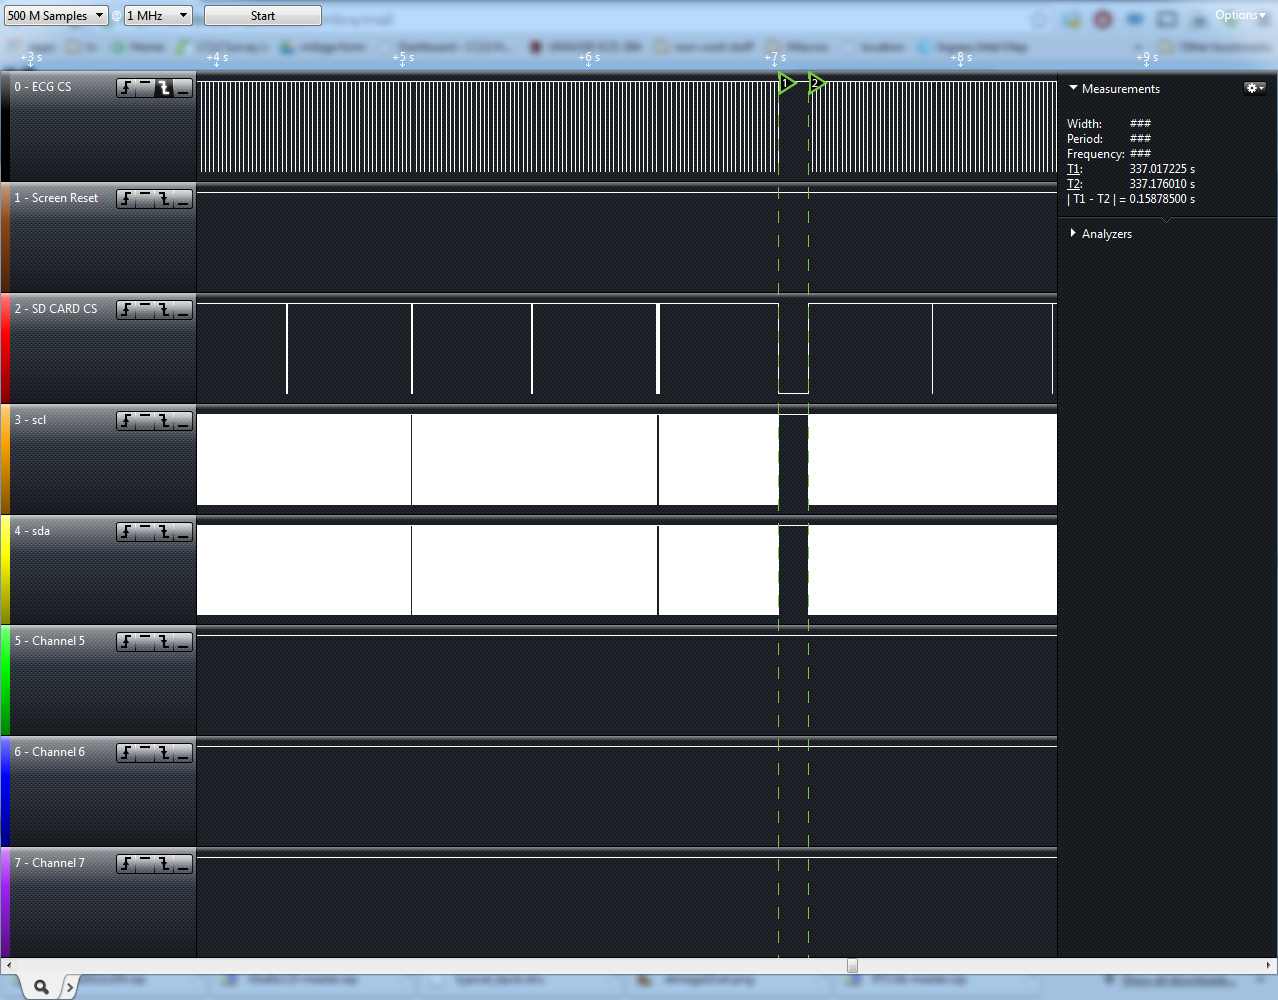
\includegraphics[scale=1,width=0.8\textwidth]{Images/logicTrace_jitter.png}
		\caption{Logic analyzer trace, time between sdCard\_ CS lows is 646mS, large sdCard\_ CS width is 158mS.}
	\end{center}
\end{figure}


\begin{figure}
	\begin{center}
		\label{fig:ecgJitterZoom}
		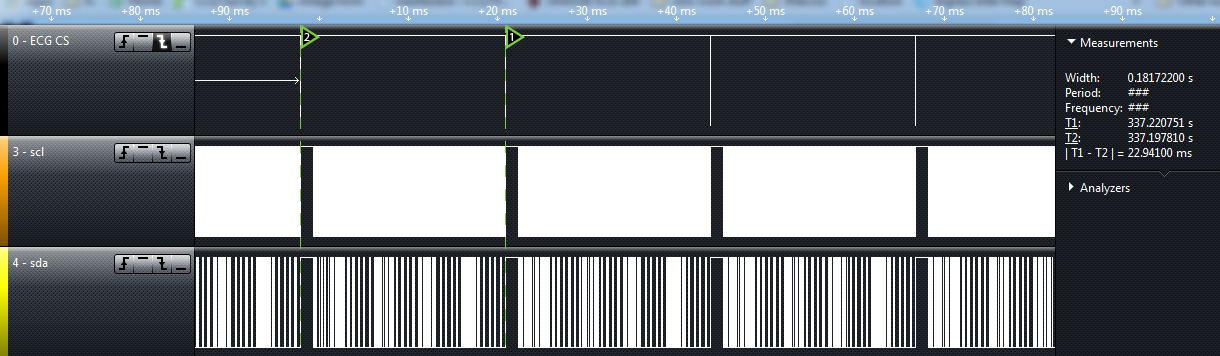
\includegraphics[scale=1,width=0.8\textwidth]{Images/logicTrace_jitter_fullScale.png}
		\caption{Logic analyzer trace, ECG sample time shown as 22mS, I2C interface shown as very active.}
	\end{center}
\end{figure}

%\begin{center}
%\newcolumntype{L}[1]{>{\hsize=#1\hsize\raggedright\arraybackslash}X}%
%\newcolumntype{R}[1]{>{\hsize=#1\hsize\raggedleft\arraybackslash}X}%
%\newcolumntype{C}[1]{>{\hsize=#1\hsize\centering\arraybackslash}X}%
%    \begin{tabularx}{\textwidth}{ |L{.9}|C{1.5}|C{.5}|C{1.1}|}
%    \hline
%    Standard 			& 		Wi-Fi 		& 		Bluetooth 	& 		ZigBee 		 \\ \hline
%    IEEE~spec. 			& 802.11 a/b/g 		& 802.15.1 			& 802.15.4 			 \\ \hline
%    Frequency~band 		& 2.4GHz; 5GHz		& 2.4GHz			& 868/915MHz; 2.4GHz \\ \hline
%    Max~Signal~Rate 	& 54 Mb/s			& 1Mb/s				& 250Kb/s			 \\ \hline
%    Nominal~range 		&100 m&10 m&10-100 m\\ \hline
%    Nominal~TX power 	&15 – 20 dBm&0-10 dBm&(-25)-0 dBm \\ \hline
%Number of RF channels &14 (2.4 GHz)&79&1/10; 16\\ \hline
%Channel bandwidth&22 MHz&1 MHz&0.3/0.6MHz; 2MHz\\ \hline
%Modulation type&BPSK, QPSK, COFDM, CCK, M-QAM&GFSK&BPSK (+ ASK), O-QPSK\\ \hline
%Spreading&DSSS, CCK, OFDM&FHSS&DSSS\\ \hline
%Coexistence mechanism&Dynamic freq. selection, transmit power control (802.11h)&Adaptive freq. hopping&Dynamic freq. selection\\ \hline
%Basic cell&BSS&Piconet&Star\\ \hline
%Extension of the basic cell&ESS&Scatternet&Cluster tree, Mesh\\ \hline
%Max \# cell nodes&2007&8&65000\\ \hline
%Encryption&RC4 stream cipher (WEP), AES block cipher&E0 stream cipher&AES block cipher (CTR, counter mode)\\ \hline
%Authentication&WPA2 (802.11i)&Shared secret&CBC-MAC (ext. of CCM)\\ \hline
%Data protection&32-bit CRC&16-bit CRC&16-bit CRC\\ \hline
%
%    \end{tabularx}
%\end{center}